\section{Durchführung}
\label{sec:Durchführung}

\subsection{Bestimmung der Zeitkonstante durch einen Ent- oder Aufladevorgang}

    Zuerst wird eine Schaltung gemäß der \autoref{fig:schaltunga} aufgebaut. Es handelt sich dabei um einen $RC$-Kreis, also eine Reihenschaltung eines Widerstandes
    und eines Kondensators. Der Kreis wird mit einer rechteckförmigen Spannung gespeist, und die Kondensatorspannugn wird abgegriffen und auf einem Oszillograph
    sichtbar gemacht. 

    \begin{figure}[H]
        \centering
        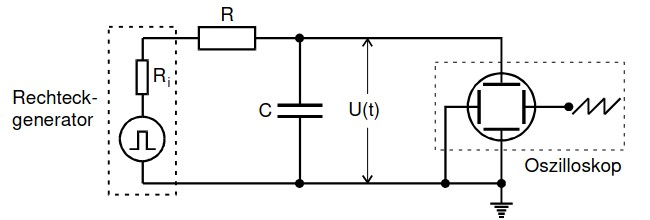
\includegraphics[width=0.6\textwidth]{bilder/aufbau_schaltunga.jpg}
        \caption{Die Schaltung zur Messung eines Ent- oder Aufladevorgangs. \cite{anleitung}}
        \label{fig:schaltunga}
    \end{figure}

    \noindent Das Oszilloskop ist so einzustellen, dass sich ein einzelner Ent- oder Aufladevorgang gut ablesen lässt, wie es in der \autoref{fig:entladekurvetheo}
    zu sehen ist.

    \begin{figure}
        \centering
        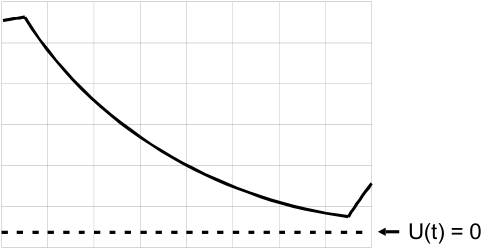
\includegraphics[width=0.6\textwidth]{bilder/Entladekurve.PNG}
        \caption{Das Beispiel eines auf einem Oszilloskop sichtbar gemachtem Entladevorgang eines Kondensators über einen Widerstand. \cite{anleitung}}
        \label{fig:entladekurvetheo}
    \end{figure}


\subsection{Bestimmung der Zeitkonstante durch die Amplitude}

    Für diese Messung wird auch der Schaltkreis gemäß \autoref{fig:schaltunga} genutzt, jedoch wird nun mit einer Sinusspannung gespeist. Nun wird die 
    Kondensatorspannung wieder auf dem Schirm des Oszillograph angezeigt und ihre Amplitude abgelesen. Die Frequenz der Sinusspannung wird von 
    $\SI{10}{\hertz}$ bis $\SI{10}{\kilo\hertz}$ variert. 


\subsection{Bestimmung der Zeitkonstante durch die Phasenverschiebung}

    Zur Messung der Zeitkonstante durch die Phasenverschiebung zwischen Speise- und Kondensatorspannung, wird ein Schaltkreis nach der \autoref{fig:schaltungc}
    aufgebaut. 

    \begin{figure}[H]
        \centering
        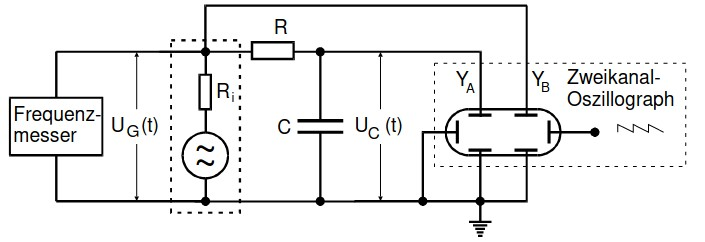
\includegraphics[width=0.6\textwidth]{bilder/aufbau_schaltungc.jpg}
        \caption{Ein Schaltkreis zur Ermittelung der Phasendifferenz zwischen Kondensator- und Speisespannung mit Hilfe eines Zweikanal-Oszilloskop. \cite{anleitung}}
        \label{fig:schaltungc}
    \end{figure}

    \noindent Es handelt sich hierbei wiedermals um einen $RC$-Kreis, welche mit einer Sinusspannung gespeist wird. Nun werden jedoch die Kondensator- und die 
    Speisespannung auf dem Oszillographenschirm angezeigt. Es sollte sich ein ähnliches Bild zu \autoref{fig:zweistrahlosz} ergeben; die Werte für $a$ und $b$
    werden notiert, wobei $b$ der Schwingungsdauer entspricht. Die Phasenverschiebung ist gegeben durch.
    \begin{equation*}
        \varphi = \frac{a}{b} \cdot 2 \pi
    \end{equation*}

    \begin{figure}
        \centerung
        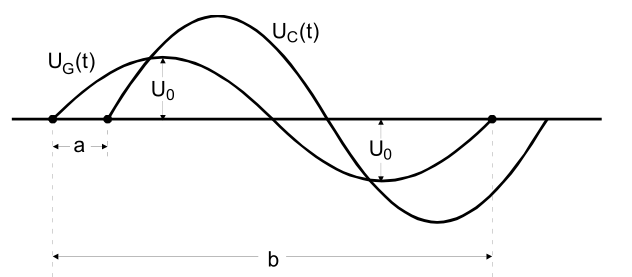
\includegraphics[width=0.6\textwidth]{bilder/Zweistrahloszillograph.PNG}
        \caption{Messung der Phasenverschiebung zwischen zwei Spannungen mit dem Zweistrahloszillographen.}
        \label{fig:zweistrahlosz}
    \end{figure}